\documentclass[12pt]{article}

\usepackage{amsfonts}
\usepackage{amsmath}
\usepackage{amssymb}
\usepackage{fancyhdr}
\usepackage[headheight=1in,margin=1in]{geometry}
\usepackage[colorlinks=true,linkcolor=blue]{hyperref}
\usepackage{mathtools}
\usepackage{tikz}

\newcommand{\N}{\mathbb{N}}
\newcommand{\Z}{\mathbb{Z}}
\newcommand{\Q}{\mathbb{Q}}
\newcommand{\R}{\mathbb{R}}
\newcommand{\C}{\mathbb{C}}
\newcommand{\F}{\mathbb{F}}

\renewcommand{\t}[1]{\text{#1}}

\newcommand{\angleb}[1]{\left\langle#1\right\rangle}
\newcommand{\braceb}[1]{\left\{#1\right\}}
\newcommand{\bracketb}[1]{\left[#1\right]}
\newcommand{\parenb}[1]{\left(#1\right)}
\newcommand{\vertb}[1]{\left\vert#1\right\vert}
\newcommand{\ovl}[1]{\overline{#1}}

\newcommand{\normsub}{\trianglelefteq}
\newcommand{\normsup}{\trianglerighteq}

\newcommand{\done}{\ensuremath{\strut\hfill\blacksquare}}

\begin{document}

\pagestyle{fancy}
\fancyhead[L]{Modern Algebra}
\fancyhead[C]{Alex Agruso}
\fancyhead[R]{Homework 4}

\setlength{\parindent}{0in}
\setlength{\parskip}{0.1in}

\section*{2.5 The Lattice of Subgroups of a Group}

\textbf{9b)}
The divisors of \( 24 \) are \( 1, 2, 3, 4, 6, 8, 12, \) and \( 24 \), so we
have that the subgroup lattice of \( \Z/24\Z \) is
\begin{center}
	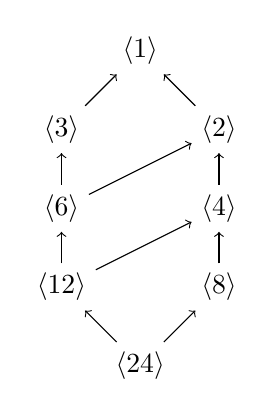
\begin{tikzpicture}
		\node (24) at (0,0)  {\( \angleb{24} \)};
		\node (12) at (-1,1) {\( \angleb{12} \)};
		\node (8)  at (1,1)  {\( \angleb{8} \)};
		\node (6)  at (-1,2) {\( \angleb{6} \)};
		\node (4)  at (1,2)  {\( \angleb{4} \)};
		\node (3)  at (-1,3) {\( \angleb{3} \)};
		\node (2)  at (1,3)  {\( \angleb{2} \)};
		\node (1)  at (0,4)  {\( \angleb{1} \)};

		\draw[->] (24) to (12);
		\draw[->] (24) to (8);
		\draw[->] (12) to (6);
		\draw[->] (12) to (4);
		\draw[->] (8)  to (4);
		\draw[->] (6)  to (3);
		\draw[->] (6)  to (2);
		\draw[->] (4)  to (2);
		\draw[->] (3)  to (1);
		\draw[->] (2)  to (1);
	\end{tikzpicture}
\end{center}

\section*{3.1 Definitions and Examples}

\textbf{1)}
Let \( \phi : G \to H \) be a homomorphism and fix a subgroup \( E \leq H \).
Since \( e' \in E \), we have \( \phi(e) = e' \), thus
\( e \in \phi^{-1}(E) \).
Now let \( a, b \in \phi^{-1}(E) \), then \( \phi(a), \phi(b) \in E \), and
thus by the closure of \( E \) we have \( \phi(a)\phi(b) = \phi(ab) \in E \),
and thus \( ab \in \phi^{-1}(E) \).
We also have that \( \phi(a)^{-1} = \phi(a^{-1}) \in E \), thus
\( a^{-1} \in \phi^{-1}(E) \), and thus \( \phi^{-1}(E) \leq G \).

Now suppose \( E \normsub H \).
Let \( h \in \phi^{-1}(E) \) and fix \( g \in G \), then
\( \phi(ghg^{-1}) = \phi(g)\phi(h)\phi(g)^{-1} \).
Since \( \phi(h) \in E \) and \( \phi(g) \in H \), we have that
\( \phi(ghg^{-1}) \in E \), thus \( ghg^{-1} \in \phi^{-1}(E) \), which proves
that \( \phi^{-1}(E) \normsub G \).

Since \( \braceb{e'} \normsub H \), we can deduce that
\( \phi^{-1}(\braceb{e'}) = \ker\phi \normsub G \).
\done

\textbf{6)}
Define \( \phi : \R^\times \to \braceb{\pm 1} \) as
\( a \mapsto a/\vertb{a} \), then we have that
\( \phi^{-1}(\braceb{1}) = (0, \infty) \) and
\( \phi^{-1}(\braceb{-1}) = (-\infty, 0) \).
Fix \( a, b \in \R^\times \), then
\[
	\phi(ab)
	= \frac{ab}{\vertb{ab}}
	= \frac{a}{\vertb{a}} \cdot \frac{b}{\vertb{b}}
	= \phi(a)\phi(b),
\]
thus \( \phi \) is a homomorphism.
\done

\textbf{10)}
Fix \( \ovl{a}, \ovl{b} \in \Z/8\Z \) with \( \ovl{a} = \ovl{b} \), then
\( a \equiv b \pmod{8} \), so we have that \( a = b + 8n \) for some
\( n \in \Z \), but then \( a = b + 4k \) with \( k = 2n \), thus
\( a \equiv b \pmod{4} \) and \( \phi(\ovl{a}) = \phi(\ovl{b}) \), showing
that \( \phi \) is well-defined.
We also have that \( \phi \) is surjective since
\( \ovl{a}_8 \mapsto \ovl{a}_4 \) for \( 1 \leq a \leq 4 \).
Finally, we have that the fibers of \( \phi \) are
\( \ker\phi = \phi^{-1}(\braceb{\ovl{1}}) = \braceb{\ovl{1}, \ovl{5}} \),
\( \phi^{-1}(\braceb{\ovl{2}}) = \braceb{\ovl{2}, \ovl{6}} \),
\( \phi^{-1}(\braceb{\ovl{3}}) = \braceb{\ovl{3}, \ovl{7}} \), and
\( \phi^{-1}(\braceb{\ovl{4}}) = \braceb{\ovl{4}, \ovl{8}} \).

\textbf{24)}
Fix a group \( G \) and subgroups \( H \) and \( N \) where \( N \normsub G \).
Given \( h \in H \) and \( a \in H \cap N \), we have by closure that
\( hah^{-1} \in H \), and since \( N \normsub G \) and \( h \in G \), we have
that \( hah^{-1} \in N \), thus \( hah^{-1} \in H \cap N \), and thus
\( H \cap N \normsub H \).
\done

\textbf{36)}
Let \( G \) be a group and suppose \( G/Z(G) \) is cyclic, then
\( G/Z(G) = \angleb{aZ(G)} \) for some \( a \in G \).
Fix \( b_1, b_2 \in G \), then \( b_1Z(G) = a^mZ(G) \) and
\( b_2Z(G) = a^nZ(G) \) for integers \( m \) and \( n \), thus
\(
	b_1b_2Z(G)
	= a^ma^nZ(G)
	= a^{m + n}Z(G)
	= a^{n + m}Z(G)
	= a^na^mZ(G)
	= b_2b_1Z(G)
\),
thus \( b_1b_2 = b_2b_1 \) and \( G \) is abelian.
\done

\textbf{40)}
Given a group \( G \) and a normal subgroup \( N \) of \( G \), let
\( \ovl{x}, \ovl{y} \in G/N \) and suppose \( \ovl{xy} = \ovl{yx} \), then
\( xyN = yxN \), thus \( xyn_1 = yxn_2 \) for some \( n_1, n_2 \in N \).
Consequently, \( x^{-1}y^{-1}xy = n_2n_1^{-1} \), thus
\( x^{-1}y^{-1}xy \in N \).
Now, assume \( x^{-1}y^{-1}xy \in N \) and fix \( n_1 \in N \), then
\( x^{-1}y^{-1}xyn_1 = n_2 \) for some \( n_2 \in N \), thus
\( xyn_1 = yxn_2 \) and \( xyN \subseteq yxN \).
We also have that \( n_1^{-1}x^{-1}y^{-1} = n_2y^{-1}x^{-1} \), for some
\( n_2 \in N \), and taking inverses we obtain \( yxn_1 = xyn_2 \), thus
\( yxN \subseteq xyN \), which shows that \( xyN = yxN \) and thus
\( \ovl{xy} = \ovl{yx } \).
\done

\section*{3.2 More on Cosets and Lagrange's Theorem}

\textbf{4)}
Let \( G \) be a group with \( \vertb{G} = pq \) for primes \( p \) and
\( q \).
Since \( Z(G) \leq G \), we have that
\( \vertb{Z(G)} \in \braceb{1, p, q, pq} \).
Clearly if \( \vertb{Z(G)} = pq \) then \( G = Z(G) \) and is abelian.
If \( \vertb{Z(G)} = 1 \), then \( Z(G) = \braceb{e} \) and we are finished.
Now let \( \vertb{Z(G)} = p \), then
\( \vertb{G/Z(G)} = \vertb{G} / \vertb{Z(G)} = pq/p = q \), and since \( q \)
is prime we have that \( G/Z(G) \) is cyclic, thus \( G \) is abelian.
A similar argument shows that \( G \) is abelian if \( \vertb{Z(G)} = q \).
\done

\textbf{8)}
Let \( H \) and \( K \) be finite subgroups of a group \( G \) where
\( (\vertb{H}, \vertb{K}) = 1 \).
We clearly have that \( e \in H \cap K \).
Now, suppose \( x \in H \) has order \( > 1 \), then \( \vertb{x} \) divides
\( \vertb{H} \), thus \( (\vertb{x}, \vertb{K}) = 1 \), and thus
\( x \notin K \).
Note that the order of an element in a subgroup is equal to its order in the
containing group.
Similarly, we have that \( (\vertb{y}, \vertb{H}) = 1 \) for any non-identity
element \( y \in K \), thus \( y \notin H \), thus \( H \cap K = \braceb{e} \).
\done

\textbf{16)}
Fix \( a \in \Z/p\Z \) and let \( \vertb{a} = k \), then
\( a^k \equiv 1 \pmod{p} \).
Since \( \vertb{\angleb{a^k}} = k \), we have by Lagrange's theorem that
\( k \mid p - 1 \), thus \( p - 1 = kn \) for some \( n \in \Z \).
Thus we have that
\( a^p = a^{kn + 1} = a^{kn}a = (a^k)^na \equiv a \pmod{p} \).
\done

\end{document}
